\chapter{Resultados}
\label{Resultados}
\section{Proceso de Desarrollo}
%explicar que el proceso de desarrollo se dividió en varias etapas
El desarrollo de Virus Breaker se dividió en varias \textbf{iteraciones} con el objetivo de reducir los riesgos del proyecto. El objetivo de cada iteración es obtener, a partir del resultado anterior, un \textbf{producto funcional} más sofisticado que el de la iteración anterior. Al planificar el desarrollo de esta forma, es más fácil adaptar el diseño a problemas detectados durante el desarrollo y además permite que, en caso de tener que detener el proceso antes de su completitud, se puede obtener un resultado mínimamente viable.

%explicar que el proyecto se vio interrumpido por causas externas en varias ocasiones
Originalmente, el proyecto se planeó en \textbf{iteraciones de un mes}. Al finalizar cada iteración, se utilizaban los datos obtenidos para planificar las iteraciones siguientes. Dividir las iteraciones en unidades de un mes permitía que las de trabajo fuesen lo unidades suficientemente pequeñas como para poder aplicar cambios en la planificación de forma efectiva, al mismo tiempo que permitía desarrollar secciones del juego lo suficientemente grandes como para poder obtener información útil sobre el progreso. 

Sin embargo, el desarrollo del proyecto tuvo que ser detenido varias ocasiones debido las exigencias de los estudios y al comienzo de las prácticas laborales. Por culpa d esto, las distintas iteraciones se encontraban separadas por \textbf{periodos de inactividad}. Esto obligó la inclusión \textbf{iteraciones de refresco} en las que el proyecto debía ser revisado para volver a familiarizarse con el código y las convenciones de desarrollo. 

Al final, las iteraciones en las que se dividió el proyecto fueron muy distintas a las planeadas en un primer momento y además tenían una duración variable. En los siguientes apartados se describen las distintas etapas del desarrollo.

\subsection{Prototipo}
%que es un prototipo y su importancia en el desarrollo de juegos
Un \textbf{prototipo} es, en el ámbito del desarrollo de videojuegos, es una implementación parcial del producto final que se utiliza para probar ideas y conceptos antes de pasar a la producción completa. El uso de prototipos permite encontrar fallos de diseño difíciles de descubrir sobre el papel sin arriesgarse a encontrarlos durante la producción, cuando su corrección sería tremendamente costosa. 

%describir prototipo creado para el juego
El prototipo de Virus Breaker consistía en los elementos básicos del juego: la pelota, el jugador, la sala y los ladrillos básicos. Todos estos elementos se encontraban reducidos a su mínima expresión con el objetivo de poder ser implementados en el menor tiempo posible. De la misma forma, el juego carecía tanto de \textbf{condición de victoria como de derrota}. Las diferencias entre esta versión y la versión definitiva son, agrandes rasgos, las siguientes:
\begin{itemize}
\item La pelota no producía ninguno de los \textbf{efectos de partículas} actuales y su comportamiento a la hora de colisionar era mucho más simple. La pelota tampoco tenía puntos de golpe, por lo que no podía ser destruida.
\item El \textbf{personaje principal} carecía de modelo (era un prisma cuadrangular) y animaciones. Aunque su movimiento era similar al actual, la paleta hacia rebotar a la pelota de forma más simplista. Tampoco podía ser derrotado ni confundido.
\item La \textbf{sala} carecía de puerta (eran cuatro paredes) y utilizaba una textura por defecto en todas sus caras. Ninguno de sus elementos tenía más comportamiento que ser sólido físicamente.
\item Solo había \textbf{un tipo de ladrillo}, el básico, que carecía de textura o efectos visuales. Su única función era la de ser destruido si lo golpeaba la pelota. Estos ladrillos se colocaban manualmente en la puerta mediante el Editor de Unity.
\item La acción del juego se desarrollaba en \textbf{una única escena}.
\item No había \textbf{interfaz gráfica de usuario}.
\end{itemize} 
Una captura de este prototipo puede verse en la figura \ref{captura_prototipo}.
\begin{figure}[h]
    \centering
    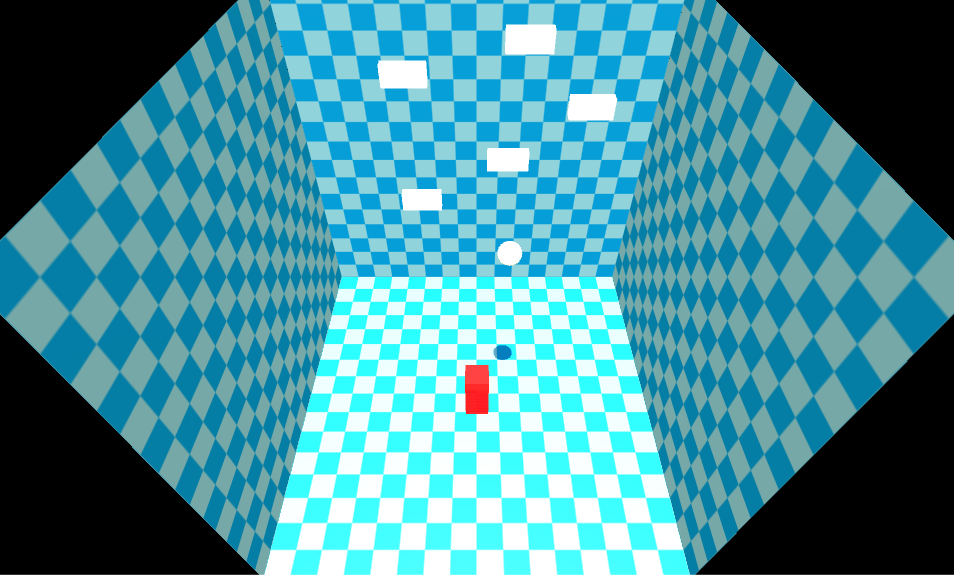
\includegraphics[width=0.8\textwidth]{images/resultados/desarrollo/prototipo}
    \caption{Captura del prototipo (Recreación).}
    \label{captura_prototipo}
\end{figure}

%que se encontró de utilidad
Esta complementación del juego fue muy útil para calcular los valores exactos de velocidad de la pelota y el jugador, importantes para lograr una sensación de juego agradable. Por otro lado, fue posible identificar unos problemas fundamentales con el movimiento de la pelota. 

En primer lugar, al rebotar con la ``puerta'', era bastante común que acabase rebotando con la pared del sur de la sala y su movimiento se volviese mucho más difícil de controlar para el jugador. En segundo lugar, era muy difícil controlar la pelota con la paleta, primero la extremada dificultad de darle (la pelota tendía a quedar entre el jugador y la paleta) y en segundo porque no había forma de controlar la dirección de salida de forma efectiva. Estos problemas pudieron ser \textbf{resueltos de forma efectiva} añadiendo cambios a los comportamientos de la pelota, el jugador y la paleta que no se encontraban en el diseño inicial. 

%resultados de la etapa y duración
El desarrollo de este prototipo duró un mes, el tiempo esperado del desarrollo esperado. El ritmo del desarrollo fue de aproximadamente un elemento por semana, aunque el personaje principal necesito de tiempo extra.

\subsection{Mecánicas de Juego Complementarias}
%explicar que se buscaba en esta etapa (versión jugable
El prototipo resultante de la etapa anterior podía considerarse lo que en diseño de juegos se conoce como \textbf{juguete} un sistema interactivo carente de objetivos \cite{clockwork_game}. Para ser considerado un juego, el jugador deberá tener \textbf{objetivos}, los cuales se alcanzarán mediante toma de \textbf{decisiones significativas}. Lejos de ser un fallo del proceso de desarrollo, comenzar implementando un juguete permite pulir correctamente su sistema de control para que sea fácil y divertido de usar. 

Por consiguiente, el objetivo será el de dotar al proyecto de los \textbf{mecánicas complementaras} que añadan objetivos. El objetivo que se eligió para el juego era el de superar todos los niveles del mismo, al mismo tiempo que se evita un \textbf{estado de derrota}. La implementación de los objetivos se realizó mediante la adición de los siguientes elementos y mecánicas:
\begin{itemize}
\item \textbf{La puerta} de la sala, y, por consiguiente, la condición de victoria del nivel.
\item \textbf{Los puntos de golpe de la pelota}, y la condición de derrota asociada a dichos puntos.
\item \textbf{Los estados adicionales del personaje principal}, es decir, el estado de confusión y el estado de derrota.
\item  \textbf{Distintos niveles} y transiciones entre ellos.
\end{itemize}

%nuevos estados
El desarrollo de esta etapa comenzó con la implementación de los nuevos estados del personaje principal, seguida de la implementación del sistema de puntos de vida de la pelota y sus correspondientes estados adicionales. Para facilitar su desarrollo, se utilizó un plugin de \textbf{máquina de estados finitos} para Unity\footnote{https://github.com/thefuntastic/Unity3d-Finite-State-Machine} que permitía dividir la ejecución de los componentes en diferentes estados.

%transiciones super básicas
En este estado, las escenas de victoria y derrota no estaban implementadas, por lo que el juego empezaba directamente en el primer nivel y, en la derrota, el nivel simplemente se reiniciaba. De la misma forma, el sistema de guardado tampoco estaba implementado, por lo que cada vez que se empezaba el juego se volvía al primer nivel.

%hablar sobre los nuevos ladrillos, los niveles, y los problemas de posición
Una vez terminados los nuevos estados, el desarrollo se centró en la construcción de niveles. Una serie de niveles fueron diseñados en papel, y después fueron implementados mediante el editor de Unity en forma de distintas escenas. Según se iban necesitando para la construcción de niveles, se implementaron el resto de los tipos de ladrillos, así como su función para asignarles colores.

Junto con los niveles, se implementó la puerta del juego con un comportamiento básico. esta disponía de puntos de vida junto con la función para realizar cambios de escena. Sin embargo, la transición entre distintas escenas era un cambio brusco debido a la falta del componente \textbf{FlashTransition} que no fue implementado hasta mucho después.

La implementación de niveles era \textbf{un proceso lento y propenso a fallos}: cada vez que se colocaba un ladrillo había que ajustar su posición a la cuadricula de forma manual lo que ralentizaba enormemente el proceso de desarrollo. De la misma forma, para los colores de los ladrillos debían ser seleccionados uno a uno y el resultado no podía verse en el editor de Unity, por lo que había que ejecutar la prueba del juego para comprobar que los ladrillos tenían los colores correctos.

En adición a estos problemas, tener los niveles implementados en distintas salas era tremendamente ineficiente ya que los cambios realizados en objetos comunes de un nivel debían ser propagados manualmente al resto de niveles. El problema se intentó paliar con el uso de \textbf{objetos prefabricados} (figura \ref{brick_prefab}), pero debido a las limitaciones de los objetos prefabricados hicieron que fuese solo una solución parcial. 
\begin{figure}[h]
    \centering
    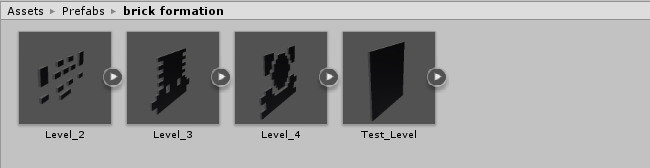
\includegraphics[width=0.8\textwidth]{images/resultados/desarrollo/brick_prefab}
    \caption{Guardar los niveles como objetos prefabricados fue una de las alternativas probadas.}
    \label{brick_prefab}
\end{figure}

%tiempo de desarrollo
La duración de esta iteración fue de dos meses, más tiempo del esperado. La causa de esta tardanza fue principalmente los problemas en la implementación de niveles. Fue en este punto donde se decidió utilizar un editor de niveles externos, ya que el incremento en el tiempo de desarrollo del sistema de carga de niveles se vería compensado por la aceleración en la implementación de niveles.

\subsection{Cambios Estéticos}
%versión pulida para presentar
El objetivo de esta iteración era la de pulir estéticamente el juego de forma que pudiese ser publicado como una \textbf{alpha abierta} en internet y así obtener feedback de usuarios. Los principales cambios añadidos en esta iteración serían texturas y modelos a los distintos objetos, efectos de sonido a las colisiones, animaciones, corrección de errores y las pantallas de inicio y final del juego.

%reacción de texturas y modelos
En primer lugar, se elaboraron \textbf{texturas para los distintos objetos}: los ladrillos, la puerta, las paredes y el personaje. Las texturas eran imágenes de baja resolución que imitaban el estilo artístico de los juegos de los años 80 y 90, no muy distintas de texturas definitivas (figura \ref{comparativa_texturas}). Mientras que la sala y los ladrillos conservaron sus simple modelos por defecto, fue necesario elaborar modelos para el personaje principal y la puerta. El personaje principal necesitaba un modelo que lo hiciese más expresivo que un simple prisma, pero la puerta necesito un modelo por cuestiones técnicas: los paneles de la puerta, a pesar de ser prismas rectangulares como por ejemplo los ladrillos, necesitaba que cada una de sus caras tuviese una textura distinta, algo difícil de implementar en los modelos por defecto de Unity. Ambos modelos fueron elaborados usando el programa \textbf{Blender3D}\footnote{www.blender.org}
\begin{figure}[!htb]
   \begin{minipage}{0.4\textwidth}
     \centering
     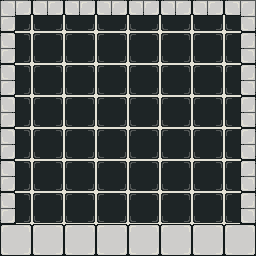
\includegraphics[width=0.9\linewidth, right]{images/resultados/desarrollo/paredes_origen}
   \end{minipage}\hfill
   \begin {minipage}{0.4\textwidth}
     \centering
     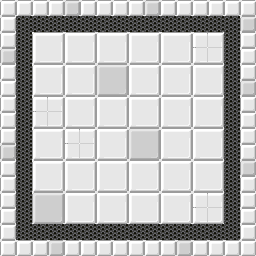
\includegraphics[width=0.9\linewidth, left]{images/resultados/desarrollo/paredes_final}
   \end{minipage}
   \caption{Comparativa entre la textura antigua (izquierda) y moderna (derecha) del suelo de la sala.}
   \label{comparativa_texturas}
\end{figure}

La pelota no recibió ningún modelo ni textura, ya que su aspecto no era muy distinto del que se buscaba, pero si se le añadieron los efectos de partículas que aún se conservan en la versión final. La paleta tampoco recibió modelo o textura, pero se ajustaron los valores de su \textbf{material} para darle un aspecto semitransparente.

%conflictos con las animaciones
El siguiente paso en esta iteración era la inclusión de \textbf{animaciones} a los distintos objetos del juego. Específicamente, el personaje principal, la pelota y la puerta fueron los objetos que recibieron animaciones nuevas para volverlos más expresivos. Sin embargo, en el proceso de adicción de animaciones se descubrió que los componentes \textbf{Animator} y \textbf{Rigidbody} entraban en conflicto debido a que ambos modificaban valores de posición y rotación de los objetos a los que estaban asignados.

Para solucionar este problema fue necesario replantear \textbf{la implementación estos objetos}, separando sus componentes en dos: un objeto principal invisible que contiene el comportamiento del objeto con un objeto asociado que se utiliza para contener los modelos y texturas. En la figura \ref{old_main_character} se puede ver el cambio realizado en el personaje principal, el cual es similar al que se aplicó a otros objetos. A pesar de parecer un cambio pequeño, la modificación de la estructura de GameObjects obligó a modificar los componentes asociados y volver a generar las animaciones.
\begin{figure}[!t]
    \centering
    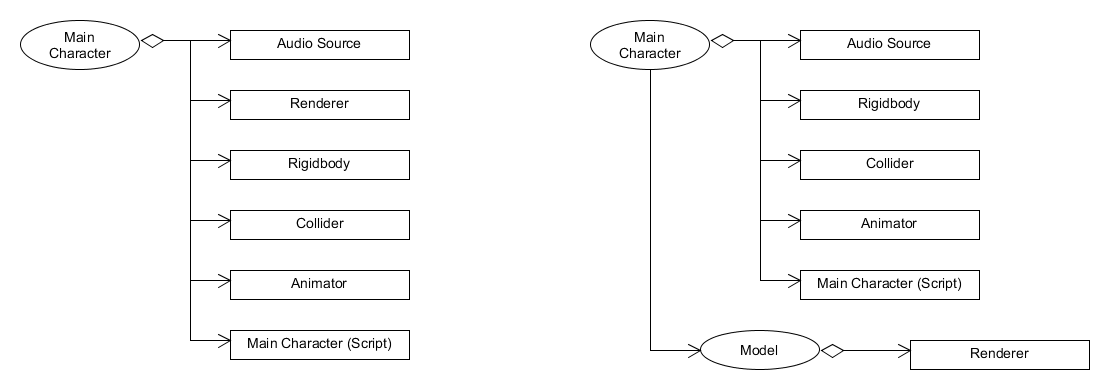
\includegraphics[width=1\textwidth]{images/resultados/desarrollo/old_main_character}
    \caption{Estructura de MainCharacter antes (izquierda) y después (derecha) de la modificación.}
    \label{old_main_character}
\end{figure}

%corrección de fallos
Aparte de los fallos causados por las animaciones, también se encontraron \textbf{fallos en la pelota y el personaje principal}. Se trataba de fallos en el cálculo de trayectoria de la pelota y en los cambios de estado del personaje principal. Solucionar estos problemas también consumió una cantidad importante de tiempo. En el proceso de revisar y corregir la pelota también se añadieron funciones para emitir efectos de sonido.

El desarrollo de esta iteración concluyo con la implementación de \textbf{las pantallas de título y de fin del juego}. En esta versión, estas pantallas estaban implementadas íntegramente mediante el sistema de interfaz de usuario de Unity, aunque su comportamiento era idéntico al actual. La figura \ref{titilo_origen} muestra cómo se veía la pantalla de título en esta versión.
\begin{figure}[h]
    \centering
    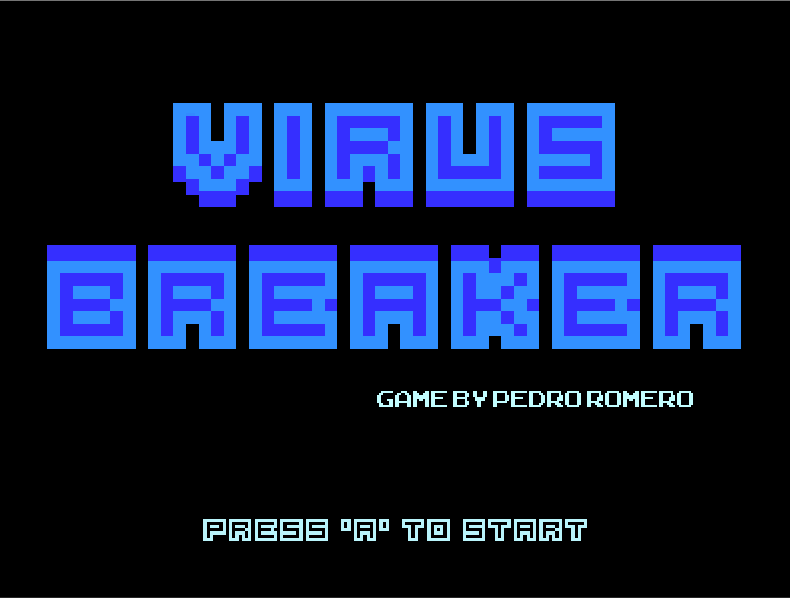
\includegraphics[width=0.8\textwidth]{images/resultados/desarrollo/titulo_origen}
    \caption{Pantalla de título antigua.}
    \label{titilo_origen}
\end{figure}

%publicación
El desarrollo de esta etapa cubrió varios meses, debido a los problemas encontrados durante su realización y a interrupciones externas. Una vez finalizada, la versión del juego obtenida en esta etapa fue publicada en la página \textbf{itch.io}\footnote{itch.io/}, un portal dedicado a la distribución de juegos. El juego fue marcado como título en desarrollo y lanzado gratis. Debido a que no se realizó mayor publicidad sobre el juego que su publicación, apenas se recibieron visitas.

\subsection{Carga de Niveles}
%refrescar causas de la implementación
%hablar del problema de usar prefabricados
El uso de una única escena de juego con un sistema de carga de nivel se eligió por encima del uso de varias escenas con diferentes configuraciones debido principalmente al gran número de elementos comunes que existen entre los distintos niveles (la geometría de la sala, el personaje, la pelota, la puerta...). De haberse optado por utilizar múltiples escenas, la repetición de elementos \textbf{supondría un gasto innecesario de recursos} y generaría problemas a la hora de realizar \textbf{modificaciones sobre los elementos comunes}, cuyos cambios tendrían que propagarse manualmente en todos los niveles.

%Tiled en profundidad
En una primera versión, se planteó el uso del programa \textbf{Tiled}\footnote{http://www.mapeditor.org/} (figura \ref{tiled}), un editor de mapas de propósito general que permite la edición de mapas basados en baldosas o \textbf{``tiles''} utilizando un sencillo procesador del lenguaje. Los mapas desarrollados generados con tiles eran exportados en formato \textbf{XML}. Para cargar los mapas en Unity se implementó un sencillo procesador del lenguaje XML que leía los ficheros y usaba su información para instanciar los ladrillos en los lugares correctos y con su color adecuado.
\begin{figure}[!t]
    \centering
    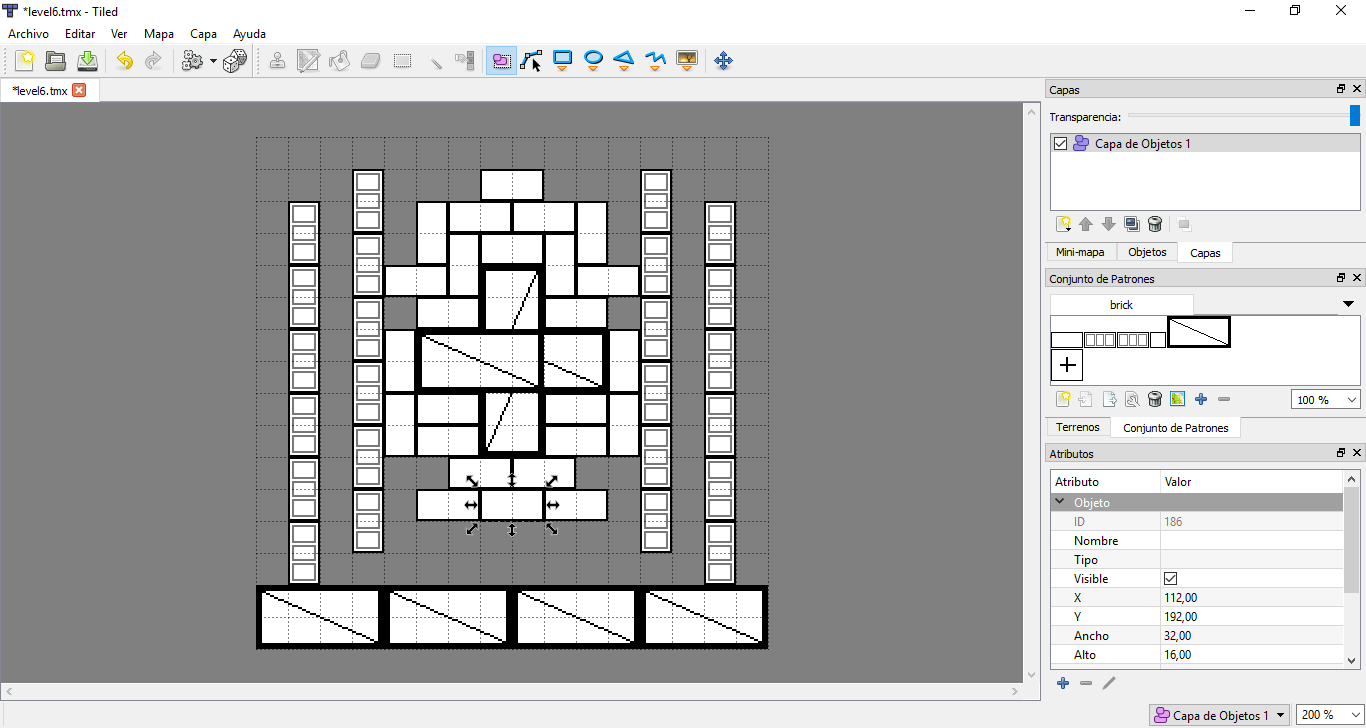
\includegraphics[width=1\textwidth]{images/resultados/desarrollo/tiled}
    \caption{Captura de Tiled durante el diseño del nivel seis del juego.}
    \label{tiled}
\end{figure}

%por qué no funcionaba
Sin embargo, utilizar Tiled \textbf{suponía varios inconveniente}s. En primer lugar, al ser un programa de propósito general, Tiled contaba con mucha \textbf{funcionalidad adicional como que resultaba innecesaria} para el proyecto y que por tanto solo ralentizaba la producción de niveles. Al mismo tiempo, este programa \textbf{carecía de cierta de ciertas funciones clave} para la elaboración del nivel. Por ejemplo, no era posible previsualizar la selección individual de colores de los ladrillos, la cual tenía que hacerse escribiendo los valores RGB del color en cada ladrillo.

%describir el proceso de la versión actual
El sistema de carga de niveles actual fue desarrollado para remplazar al sistema basado en Tiled, ya que se el tiempo de desarrollo del nuevo sistema sería menor que el de terminar todos los niveles con el sistema antiguo. Junto con el nuevo sistema, también se aisló la carga de niveles del resto de la funcionalidad de la sala creando dos componentes: \textbf{LevelGenerator} para la carga de niveles y \textbf{Room} para la coordinación de los elementos de la sala. La figura \ref{level_generator_comparation} muestra con exactitud como se produjo esta división.
\begin{figure}[h]
    \centering
    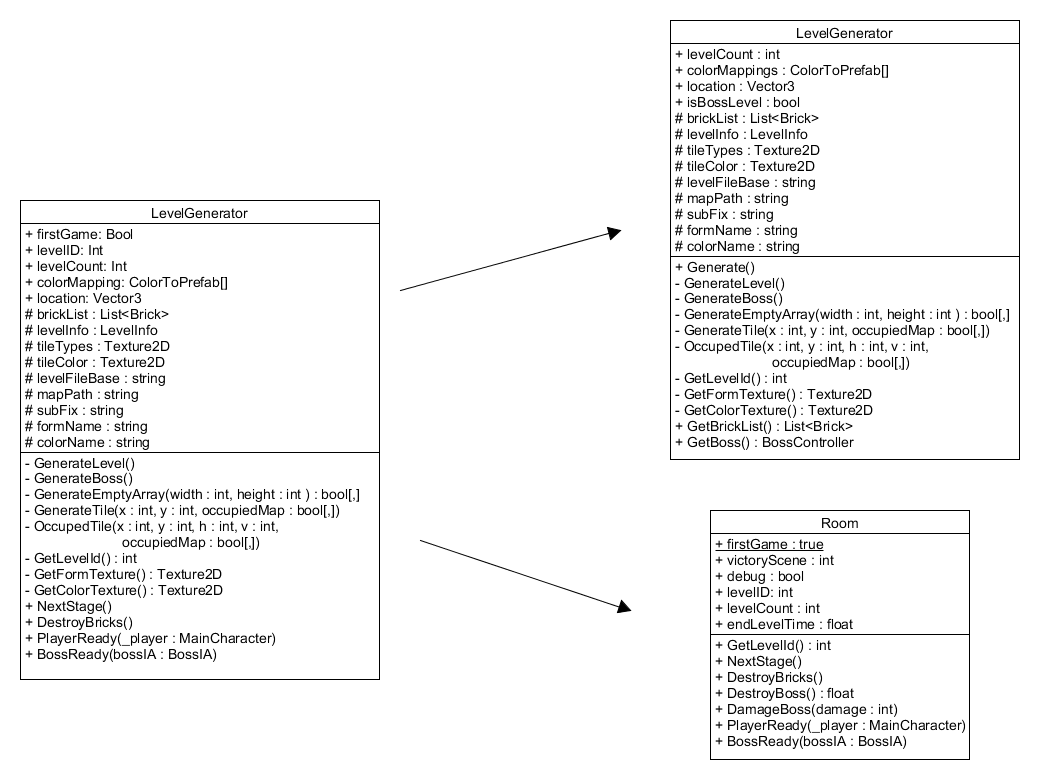
\includegraphics[width=0.8\textwidth]{images/resultados/desarrollo/level_generator_comparation}
    \caption{Extracción de la funcionalidad de la sala de LevelGenerator.}
    \label{level_generator_comparation}
\end{figure}

%tiempo (dividido en dos secciones
Ambas iteraciones del sistema de carga de niveles se completaron en aproximadamente un mes (cada una). Entre ambas iteraciones hubo un periodo largo de inactividad.

\subsection{Jefe Final}
%hablar sobre la concepción del jefe
Durante el diseño del juego, se plantearon varias \textbf{mecánicas adicionales} que serían añadidas una vez las mecánicas básicas fuesen implementadas para ampliar dar más variedad al juego. Debido a las limitaciones de tiempo del proyecto, solo una de las mecánicas adicionales podría ser implementadas. Al final se decidió implementar un jefe final para el juego.

Una vez decidido que la mecánica escogida seria la implementación de un jefe final, se diseñaron varios posibles jefes para el juego. El coste en tiempo de implementar un jefe obligaba a elegir a un solo jefe para el juego, por lo que el resto de los jefes fueron descartados una vez que se eligió al jefe actual. Estos jefes descartados eran:
\begin{itemize}
\item Un \textbf{Ciempiés gigante}, el cual se movía por las paredes y suelos de la sala de forma pseudoaleatoria entorpeciendo al jugador. Tendría una inteligencia artificial que le permitiría moverse sin nunca colisionar con su propio cuerpo.
\item Una \textbf{Figura hecha de ladrillos}. Este jefe funcionaba de forma opuesta al actual, moviéndose para evitar que la pelota golpeara sus ladrillos, ya que el jugador ganaba si le golpeaba suficientes veces.
\item Un \textbf{Mago}, el cual no interaccionaba directamente con el jugador, pero podía dificultar la partida del jugador reparando ladrillos y desviando la pelota.
\end{itemize}

En la primera etapa de su desarrollo, el comportamiento del jefe se modeló como un único componente \textbf{Boss}. Esta implementación estaba plagada de errores, el más notable era que el jefe se ``despegaba'' de la puerta a la hora de buscar la pelota. Al tratarse de un diseño monolítico, era casi imposible aislar el error, ya que podía ser a causa de una implementación incorrecta del movimiento o de un cálculo equivocado de la dirección. 

Este problema obligó a descartar la implantación del jefe y remplazarla por la estructura en dos componentes que se utiliza en la versión final. El desarrollo comenzó con la implementación de \textbf{BossController}, el componente con que modela el movimiento del jefe. Para realizar pruebas, se utilizaba un componente de pruebas que permitía enviar ordenes de movimiento a BossController mediante pulsaciones del teclado. Una vez asegurado que el movimiento carecía de fallos, se implementó la inteligencia artificial del jefe en el componente \textbf{BossIA}.

%adaptaciones cinemáticas
Una vez finalizado el comportamiento básico del jefe, se decidió darle una \textbf{animación de entrada en la sala y otra de derrota}, para volverlo más espectacular. A raíz de esta decisión, se elaboró también una secuencia de introducción, victoria y derrota general para todos los niveles del juego. Este sistema se montó por encima de otros eventos que ocurrían al principio y final del juego, como la carga del nivel o la animación de destrucción de la pelota.

%larga duración de esta etapa
Debido a la dificultad de implementar el jefe final, el problema con la implementación inicial que obligó a volver a implementar todo el sistema y la complicada integración con el resto del juego, esta iteración fue muy larga, ocupando varios meses.

\subsection{Ajustes, Refactorización y Correcciones}
%correcciones y depuración para la versión final
El objetivo de esta etapa era el de corregir el código del juego y terminar los gráficos definitivos para así poder lanzar la versión final.

%corrección de errores de programación
La corrección del código consistió en una \textbf{revisión completa} de todas las clases que lo componían para arreglar todos los fallos de programación que habían pasado desapercibidos en las etapas anteriores. La mayor parte de los fallos detectados fueron errores en las transacciones entre estados y en las llamadas entre distintos objetos. Cambien se ajustó la interfaz gráfica de usuario, que no funcionaba correctamente en todas las resoluciones.

%reorganización de las clases
Además de la corrección de errores, la revisión sirvió para \textbf{reorganizar y limpiar el código} del juego para hacerlo más comprensible. La limpieza se realizó principalmente para poder realizar labores de mantenimiento de forma más eficiente. Algunos de los cambios fueron:
\begin{itemize}
\item \textbf{Reorganización de clases}: diversas clases fueron modificadas para que su comportamiento fuese más entendible. El caso más notable fue el de la clase \textbf{Brick}, cuyas clases hijas fueron completamente reorganizadas, como puede verse en la figura \}.
\item \textbf{Estandarización de nombres} de métodos y variables: Los nombres de las clases, métodos y variables del código fueron modificados para ser adaptados al estilo de escritura \textbf{Camel Case} que es el estándar de Unity.
\item \textbf{Refactorización del código} para mejorar su eficiencia: durante la revisión se modificaron partes del código que, sin ser incorrectas, disminuían el rendimiento del programa.
\end{itemize}
\begin{figure}[!t]
    \centering
    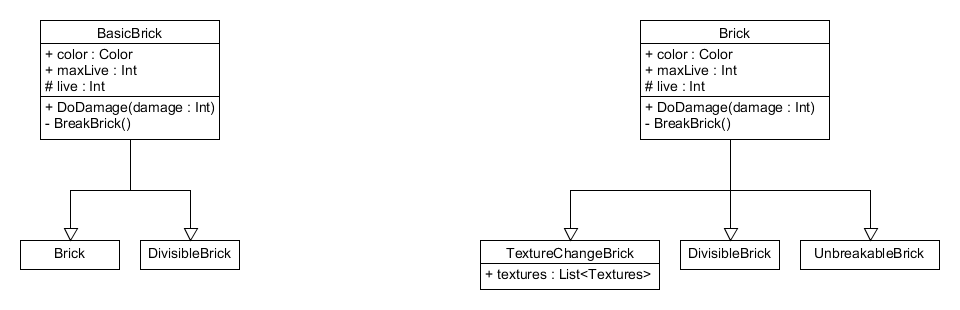
\includegraphics[width=1\textwidth]{images/resultados/desarrollo/bick_comparation}
    \caption{Jerarquía de la clase Brick antes (izquierda) y después (derecha) de la refactorización.}
    \label{bick_comparation}
\end{figure}

%texturas definitivas
Las nuevas texturas fueron elaboradas una vez terminó la limpieza del código. El objetivo del cambio de las texturas era el de \textbf{aumentar el contraste entre la sala y los elementos contenidos en ella}. El principal cambio se realizó en las texturas de la sala, que fueron completamente rediseñadas para tener un color más claro. Cambios menores fueron aplicados a las texturas del personaje principal para darles un color más saturado que contrastara mejor con el nuevo fondo claro. 
\begin{figure}[!htb]
   \begin{minipage}{0.4\textwidth}
     \centering
     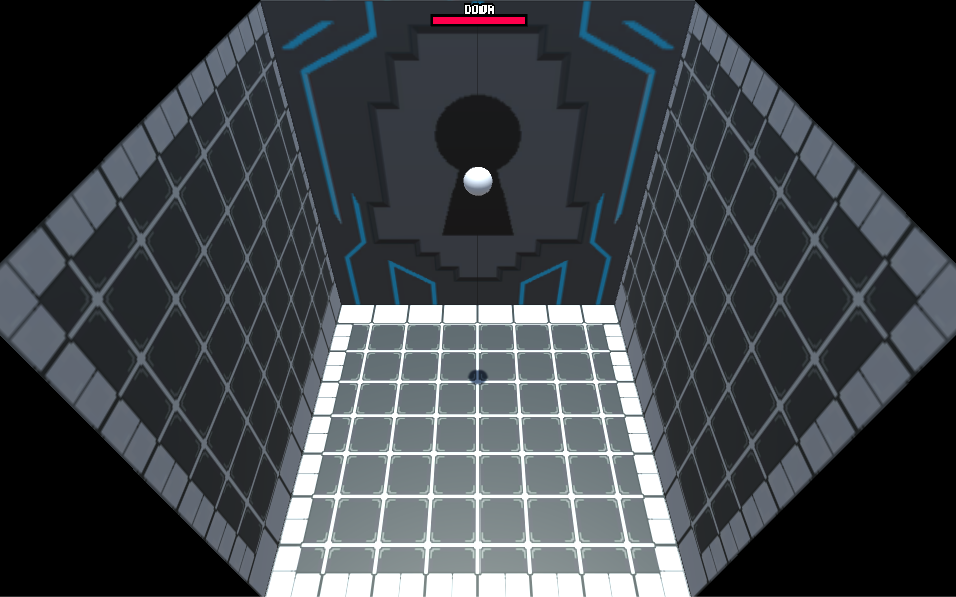
\includegraphics[width=0.9\linewidth, right]{images/resultados/desarrollo/sala_antigua}
   \end{minipage}\hfill
   \begin {minipage}{0.4\textwidth}
     \centering
     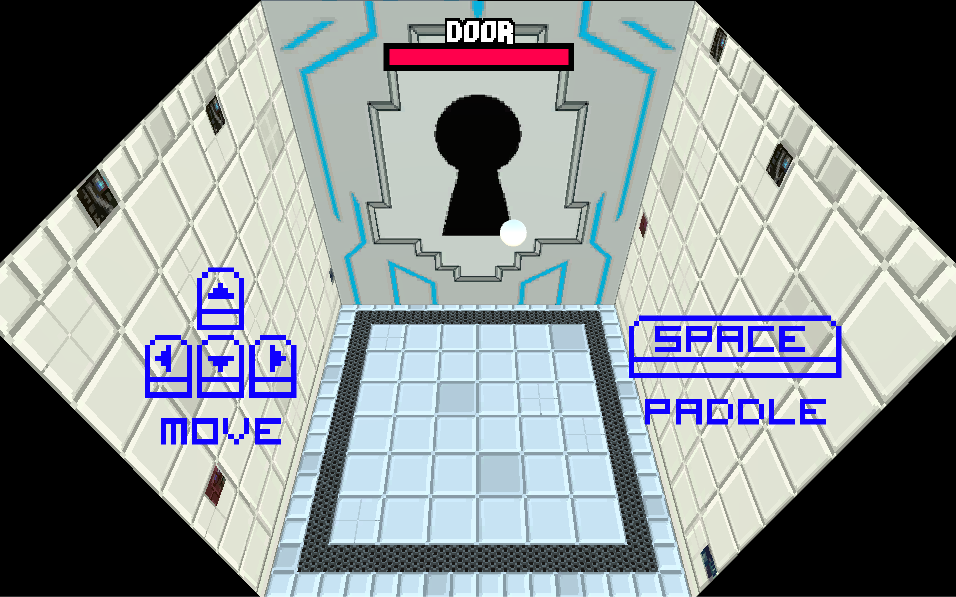
\includegraphics[width=0.9\linewidth, left]{images/resultados/desarrollo/sala_nueva}
   \end{minipage}
   \caption{Comparativa de la sala antes (izquierda) y después (derecha) de los ajustes gráficos.}
   \label{comparativa_salas}
\end{figure}

Los \textbf{valores de iluminación de la escena} de juego también fueron modificados para obtener un mejor contraste entre colores. Los cambios en la iluminación redujeron la visibilidad de la sombra de la pelota, la cual es importante para guiar al jugador, por lo que fue necesario añadir a la pelota un componente \textbf{Proyector} para emitir una sombra artificial sobre el suelo.

Esta iteración duró aproximadamente un mes y sirvió como conclusión del desarrollo. La versión final producida fue publicada en itch.io y en gamesjolt.com, acompañadas de una encuesta de opinión.

\section{Encuesta de Opinión}
Para poder obtener información sobre la opinión de los jugadores acerca del juego se elaboró una \textbf{encuesta de opinión}. Esta encuesta se compone de una serie de preguntas sobre las distintas áreas del juego, así como sobre el usuario que permitirán no solo valorar la calidad del producto de forma objetiva sino también determinar el \textbf{público objetivo} del juego.

\subsection{Descripción}
%herramienta utilizada
Para la elaboración de la encuesta se utilizó la herramienta \textbf{Google Forms}\footnote{https://docs.google.com/forms} del paquete de ofimática en line de Google. Esta herramienta permite elaborar formularios y encuestas de forma sencilla, los cuales pueden ser distribuidos por correo electrónico o mediante un enlace URL. El método de distribución mediante enlaces directos fue el utilizado para este formulario.

%falta de plantilla estándar
La \textbf{estructura de preguntas} de la encuesta tuvo que ser desarrollada desde cero al no existir ningún tipo de estándar o plantilla. Sin embargo, se utilizaron formularios similares desarrollados para otros juegos  como base, analizando sus estructuras y utilizando las preguntas más recurrentes o que mejor se adaptaban al juego. La encuesta puede dividirse en dos secciones: las preguntas sobre el jugador y las preguntas sobre la experiencia del juego.

%secciones y motivo de inclusión
La primera parte de la encuesta está dedicada a preguntas acerca de la persona encuestada. Estas preguntas servirán para discernir a que \textbf{grupo de jugadores} pertenece el encuestado, lo que nos permitirá clasificar las respuestas. Las preguntas de esta parte son:
\begin{enumerate}
\item \textbf{Genero} del encuestado.
\item \textbf{Grupo de edad} del encuestado. Los posibles grupos de edad son:
\begin{itemize}
\item Menor de 13.
\item Entre 13 y 17.
\item Entre 18 y 24.
\item Entre 25 y 34.
\item Entre 35 y 54.
\item Mayor de 55.
\end{itemize}
\item \textbf{Frecuencia de Juego} del encuestado. los posibles grupos de frecuencias son: 
\begin{itemize}
\item Todos los días.
\item Un par de veces por semana.
\item Un par de veces al mes.
\item Una vez cada varios meses.
\end{itemize}
\end{enumerate}

La segunda parte de la encuesta está formada por preguntas referentes a la \textbf{opinión sobre el juego} del encuestado. Estas preguntas son:
\begin{enumerate}
\item \textbf{¿Te pareció divertido el juego?}. La pregunta pide una valoración en una escala de 1 a 10.
\item \textbf{¿Te resultaron intuitivos los controles?}. La pregunta pide una valoración en una escala de 1 a 10.
\item \textbf{Valora la dificultad del juego}. La pregunta pide una valoración en una escala de 1 (muy fácil) a 10 (muy difícil).
\item \textbf{¿Te gustó el estilo gráfico del juego?}. La pregunta pide una valoración en una escala de 1 a 10.
\item \textbf{¿Te gustó la música y sonidos del juego?}. La pregunta pide una valoración en una escala de 1 a 10.
\item \textbf{¿Cuantos niveles superaste?}. La pregunta se responde con un campo de texto. idealmente, la respuesta será un número.
\item \textbf{¿Que te pareció la duración del juego?}. La pregunta pide una valoración en una escala de 1 a 10.
\item \textbf{¿Encontraste algún problema o error en el juego?}. La pregunta se responde con un campo de texto. Al encuestado se le pide que describa el error en caso de haber encontrado alguno.
\item \textbf{¿Comentario o sugerencia adicional?}. Esta pregunta es un espacio libre para que el encuestado exprese las opiniones que no encajen en otras secciones.
\end{enumerate}

%distribución 
El enlace a este cuestionario fue publicado en la descripción del juego en sus dos páginas de distribución. También se publicó el enlace en las redes sociales Twitter y Reddit. Adicionalmente, el enlace fue distribuido por el grupo de contactos personales del desarrollador. Para cubrir un público mayor, la encuesta se redactó en español y en inglés.

\subsection{Resultados}
%citar falta de resultados
Los resultados de la encuesta \textbf{no resultaron ser tan útiles como se esperaba}. Sumando todos los medios de distribución, solo se obtuvieron 8 votos, una cantidad demasiado pequeña como para poder realizar un estudio que resulte.

De todas formas, a modo de práctica, \textbf{se realizará un análisis de los datos obtenidos} en la encuesta. El análisis se dividirá en tres secciones: la determinación del público del juego, el análisis de la opinión de los jugadores y la reseña de las quejas y peticiones más recurrentes.

\subsubsection{Audiencia}
%descripción de la audiencia
Los datos obtenidos apuntan a que el público del juego es varones (75\% de los encuestados), de edades comprendidas entre los 13 y los 24 años, siendo ligeramente más común la franja de edad de entre 13 y 17 años (62 \% de los encuestados). Las tablas de la figura \ref{genero_edad} contienen estos datos. Estas cifras encajan con el perfil tradicional de jugador de videojuegos. 
\begin{figure}[!t]
   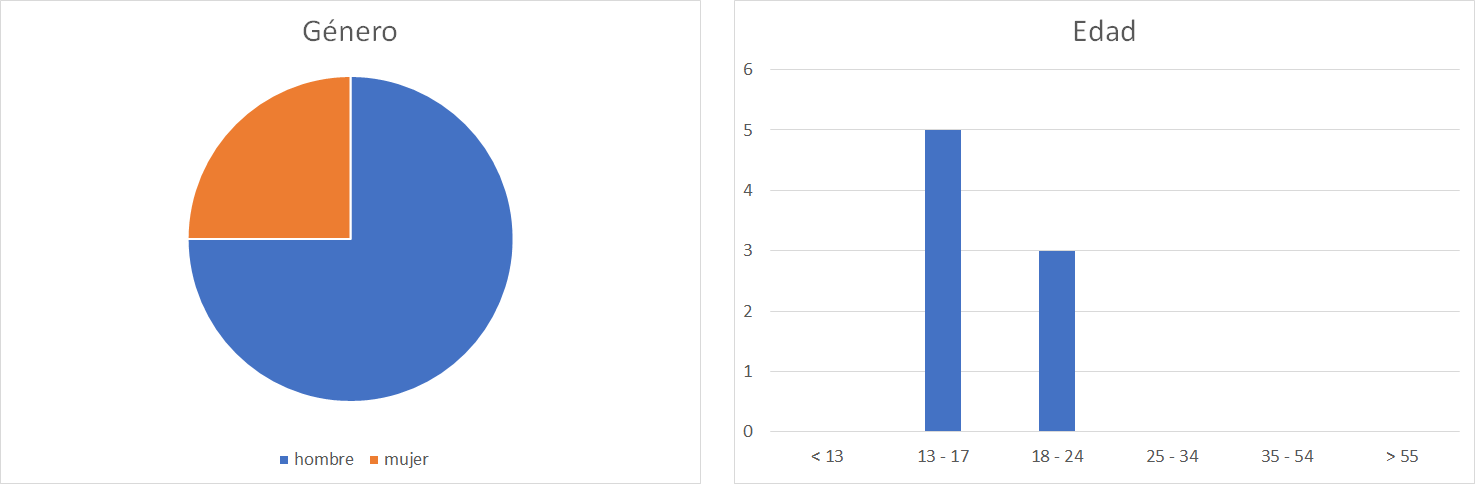
\includegraphics[width=1\linewidth, left]{images/resultados/encuesta/publico}
   \caption{Diagramas del género (izquierda) y edad (derecha).}
   \label{genero_edad}
\end{figure}

La gran mayoría de los encuestados (87.5\%) tienen una frecuencia de juego muy alta, con un 37.5\% que juega de forma diaria a algún tipo de videojuego. En la figura \ref{tabla_frecuencia} están representados estos datos.
\begin{figure}[!t]
   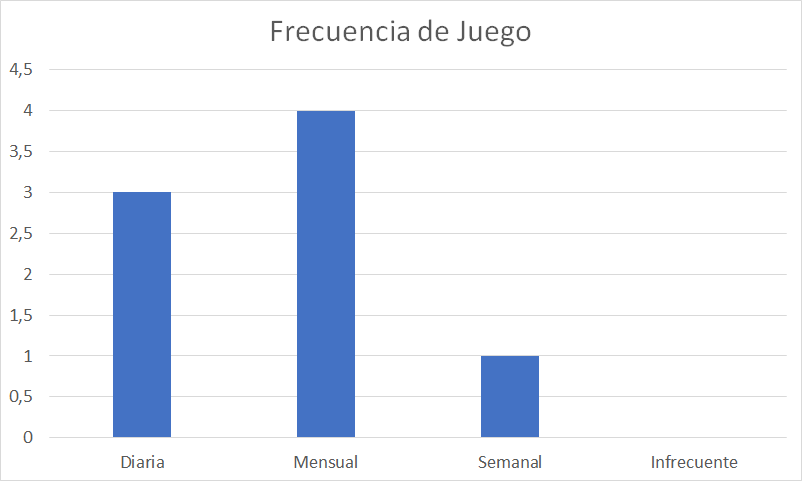
\includegraphics[width=1\linewidth, left]{images/resultados/encuesta/frecuencia}
   \caption{Diagramas de la frecuencia de juego.}
   \label{tabla_frecuencia}
\end{figure}

\subsubsection{Opinión}
%opinión sobre el juego
Los \textbf{resultados de la encuesta de opinión} se pueden ver en la figura \ref{tabla_opinion}. En esta tabla se puede apreciar como la todos los encuestados valoraron el juego de forma muy positiva, con ningún campo valorado por debajo de los cinco puntos. En promedio, la nota del juego contando todos sus apartados es de 8.7 puntos, recibiendo la nota media más baja los controles (8.25) y la más alta el apartado sonoro (9.25).
\begin{figure}[!t]
   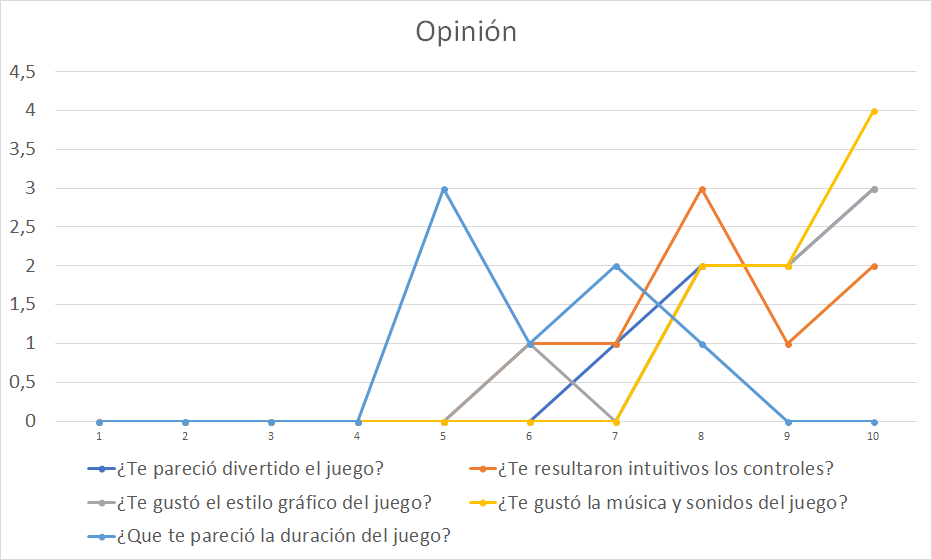
\includegraphics[width=1\linewidth, left]{images/resultados/encuesta/opinion}
   \caption{Diagrama de la opinión.}
   \label{tabla_opinion}
\end{figure}

La \textbf{opinión sobre la dificultad} debe ser valorada independientemente, ya que los mejores resultados serían las notas cercanas a los cinco puntos. En la figura \ref{tabla_dificultad} se aprecia como la mayor parte de las notas se encuentran cerca de los cinco puntos, aunque un porcentaje significativo supera este valor, dando una nota media de 6.14 puntos.
\begin{figure}[!t]
   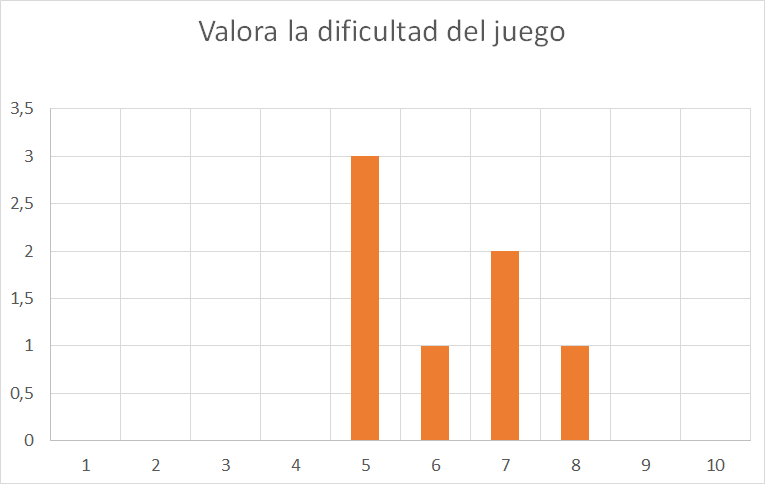
\includegraphics[width=0.9\linewidth, left]{images/resultados/encuesta/dificultad}
   \caption{Diagramas de la dificultad.}
   \label{tabla_dificultad}
\end{figure}

La cantidad de niveles superados por los encuestados se muestra en la figura \ref{tabla_niveles} indica que 78\% d de los jugadores no consiguieron terminar el juego, siendo el nivel cuatro el principal punto donde los jugadores dejaban el juego (18\% de los encuestados).
\begin{figure}[!t]
   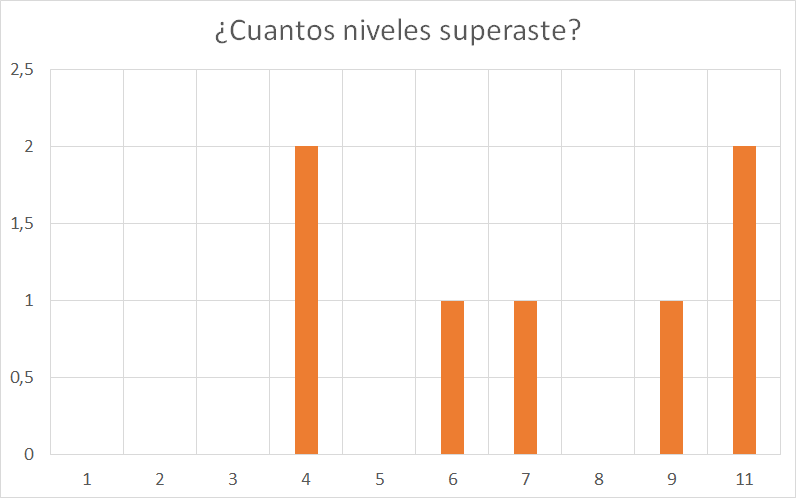
\includegraphics[width=0.9\linewidth, left]{images/resultados/encuesta/niveles}
   \caption{Diagramas de niveles superados.}
   \label{tabla_niveles}
\end{figure}

En cuanto a las quejas y sugerencias, varios usuarios indicaron que tenían problemas con los controles del juego, específicamente con la \textbf{activación de la paleta}. Otro usuario indico que en la versión actual del juego no existe ninguna forma de gestionar las \textbf{partidas guardadas}.

\subsubsection{Conclusiones}
Los resultados de la encuesta indican que el juego ha tenido una recepción positiva entre los encuestados, los cuales lo han valorado positivamente en la mayoría de las categorías analizadas.

La encuesta también ha señala a un problema en el \textbf{control de la paleta del personaje principal}, tanto mediante comentarios directos de los jugadores como con una nota menor en el apartado de controles del juego. Un control impreciso puede ser también la causa de el gran número de jugadores que no terminaron el juego y también de la dificultad elevada.
